\documentclass{standalone}
\usepackage{tikz}
\usetikzlibrary{patterns, positioning}

\begin{document}
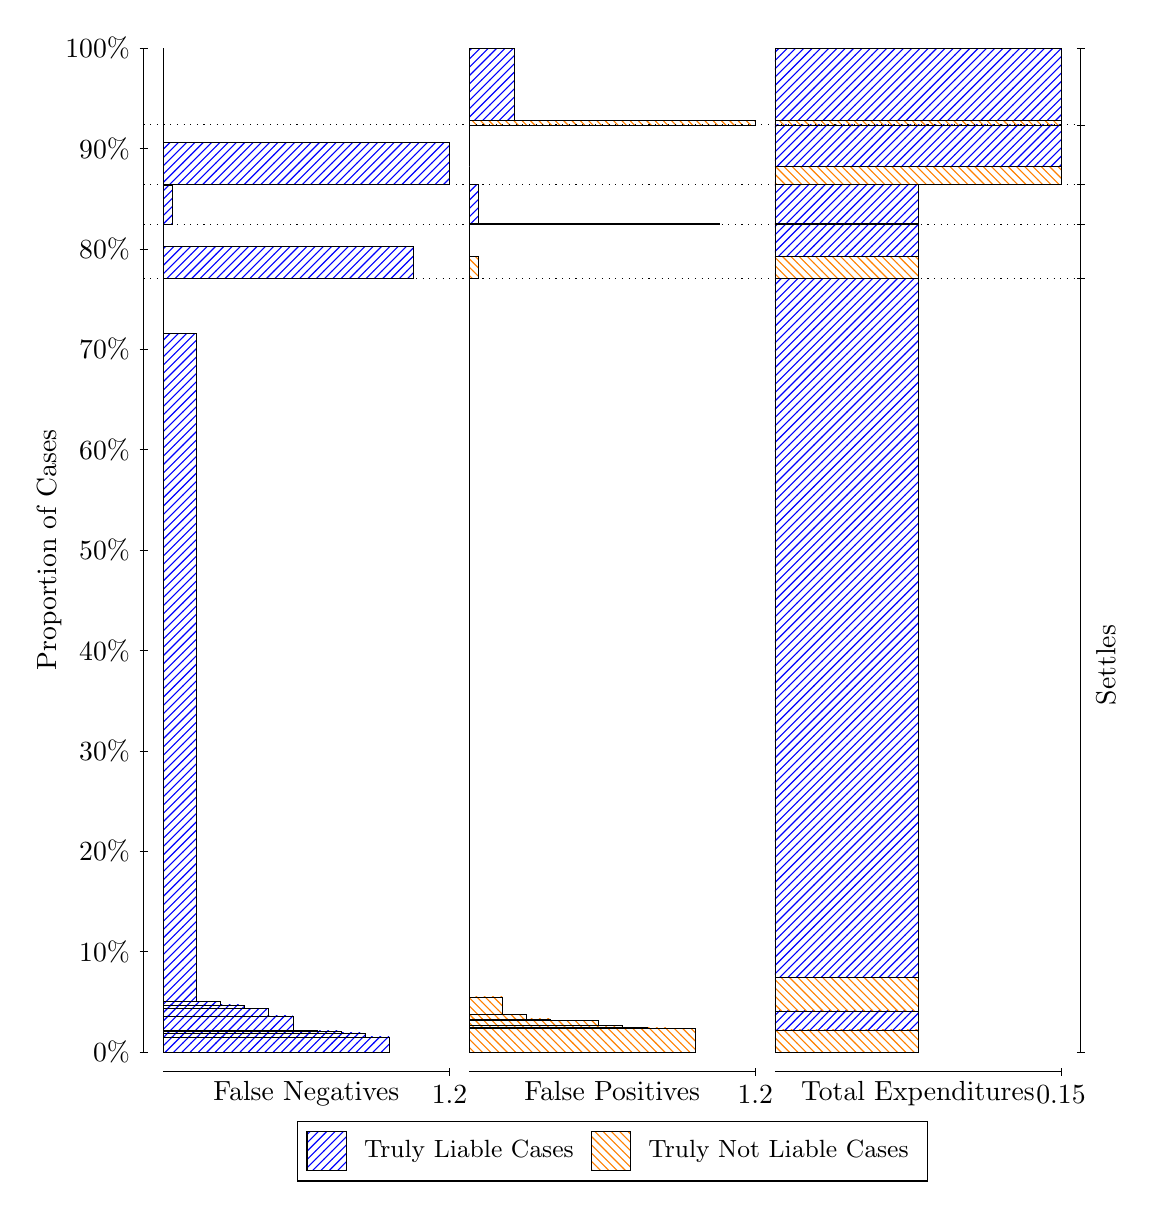
\begin{tikzpicture}
\draw[black, very thin] (1.5,1.75) -- (1.5,14.5);
\node[rotate=90, anchor=center] at (0.3, 8.125) {Proportion of Cases};
\draw[black, very thin] (1.45,1.75) -- (1.55,1.75);
\node[anchor=east] at (1.45, 1.75) {0\%};
\draw[black, very thin] (1.45,3.025) -- (1.55,3.025);
\node[anchor=east] at (1.45, 3.025) {10\%};
\draw[black, very thin] (1.45,4.3) -- (1.55,4.3);
\node[anchor=east] at (1.45, 4.3) {20\%};
\draw[black, very thin] (1.45,5.575) -- (1.55,5.575);
\node[anchor=east] at (1.45, 5.575) {30\%};
\draw[black, very thin] (1.45,6.85) -- (1.55,6.85);
\node[anchor=east] at (1.45, 6.85) {40\%};
\draw[black, very thin] (1.45,8.125) -- (1.55,8.125);
\node[anchor=east] at (1.45, 8.125) {50\%};
\draw[black, very thin] (1.45,9.4) -- (1.55,9.4);
\node[anchor=east] at (1.45, 9.4) {60\%};
\draw[black, very thin] (1.45,10.675) -- (1.55,10.675);
\node[anchor=east] at (1.45, 10.675) {70\%};
\draw[black, very thin] (1.45,11.95) -- (1.55,11.95);
\node[anchor=east] at (1.45, 11.95) {80\%};
\draw[black, very thin] (1.45,13.225) -- (1.55,13.225);
\node[anchor=east] at (1.45, 13.225) {90\%};
\draw[black, very thin] (1.45,14.5) -- (1.55,14.5);
\node[anchor=east] at (1.45, 14.5) {100\%};

\draw[black, very thin] (13.4,1.75) -- (13.4,14.5);
\draw[black, very thin] (13.35,1.75) -- (13.45,1.75);
\node[anchor=west] at (13.35, 1.75) {};
\draw[black, very thin] (13.35,11.578) -- (13.45,11.578);
\node[anchor=west] at (13.35, 11.578) {};
\draw[black, very thin] (13.35,12.257) -- (13.45,12.257);
\node[anchor=west] at (13.35, 12.257) {};
\draw[black, very thin] (13.35,12.771) -- (13.45,12.771);
\node[anchor=west] at (13.35, 12.771) {};
\draw[black, very thin] (13.35,13.524) -- (13.45,13.524);
\node[anchor=west] at (13.35, 13.524) {};
\draw[black, very thin] (13.35,14.5) -- (13.45,14.5);
\node[anchor=west] at (13.35, 14.5) {};

\draw[black, very thin, pattern color=blue, pattern=north east lines] (1.75,1.75) rectangle (4.6184,1.9412);
\draw[black, very thin, pattern color=blue, pattern=north east lines] (1.75,1.9412) rectangle (4.3125,1.9922);
\draw[black, very thin, pattern color=blue, pattern=north east lines] (1.75,1.9922) rectangle (4.0065,2.0181);
\draw[black, very thin, pattern color=blue, pattern=north east lines] (1.75,2.0181) rectangle (3.7005,2.0252);
\draw[black, very thin, pattern color=blue, pattern=north east lines] (1.75,2.0252) rectangle (3.3946,2.2087);
\draw[black, very thin, pattern color=blue, pattern=north east lines] (1.75,2.2087) rectangle (3.0886,2.305);
\draw[black, very thin, pattern color=blue, pattern=north east lines] (1.75,2.305) rectangle (2.7826,2.348);
\draw[black, very thin, pattern color=blue, pattern=north east lines] (1.75,2.348) rectangle (2.4767,2.3904);
\draw[black, very thin, pattern color=blue, pattern=north east lines] (1.75,2.3904) rectangle (2.1707,10.877);
\draw[black, very thin, pattern color=orange, pattern=north west lines] (1.75,10.877) rectangle (1.75,11.578);
\draw[black, very thin, pattern color=blue, pattern=north east lines] (1.75,11.578) rectangle (4.9244,11.977);
\draw[black, very thin, pattern color=orange, pattern=north west lines] (1.75,11.977) rectangle (1.75,12.257);
\draw[black, very thin, pattern color=blue, pattern=north east lines] (1.75,12.257) rectangle (1.8647,12.757);
\draw[black, very thin, pattern color=orange, pattern=north west lines] (1.75,12.757) rectangle (1.75,12.771);
\draw[black, very thin, pattern color=blue, pattern=north east lines] (1.75,12.771) rectangle (5.3833,13.302);
\draw[black, very thin, pattern color=orange, pattern=north west lines] (1.75,13.302) rectangle (1.75,13.524);
\draw[black, very thin, pattern color=orange, pattern=north west lines] (1.75,13.524) rectangle (1.75,13.583);
\draw[black, very thin, pattern color=blue, pattern=north east lines] (1.75,13.583) rectangle (1.75,14.5);
\draw[black, very thin, pattern color=orange, pattern=north west lines] (5.6333,1.75) rectangle (8.5018,2.0468);
\draw[black, very thin, pattern color=orange, pattern=north west lines] (5.6333,2.0468) rectangle (8.1958,2.0556);
\draw[black, very thin, pattern color=orange, pattern=north west lines] (5.6333,2.0556) rectangle (7.8898,2.0644);
\draw[black, very thin, pattern color=orange, pattern=north west lines] (5.6333,2.0644) rectangle (7.5839,2.0887);
\draw[black, very thin, pattern color=orange, pattern=north west lines] (5.6333,2.0887) rectangle (7.2779,2.1495);
\draw[black, very thin, pattern color=orange, pattern=north west lines] (5.6333,2.1495) rectangle (6.9719,2.1499);
\draw[black, very thin, pattern color=orange, pattern=north west lines] (5.6333,2.1499) rectangle (6.9719,2.1507);
\draw[black, very thin, pattern color=orange, pattern=north west lines] (5.6333,2.1507) rectangle (6.666,2.1714);
\draw[black, very thin, pattern color=orange, pattern=north west lines] (5.6333,2.1714) rectangle (6.36,2.2278);
\draw[black, very thin, pattern color=orange, pattern=north west lines] (5.6333,2.2278) rectangle (6.054,2.4507);
\draw[black, very thin, pattern color=blue, pattern=north east lines] (5.6333,2.4507) rectangle (5.6333,11.578);
\draw[black, very thin, pattern color=orange, pattern=north west lines] (5.6333,11.578) rectangle (5.7481,11.858);
\draw[black, very thin, pattern color=blue, pattern=north east lines] (5.6333,11.858) rectangle (5.6333,12.257);
\draw[black, very thin, pattern color=orange, pattern=north west lines] (5.6333,12.257) rectangle (8.8077,12.271);
\draw[black, very thin, pattern color=blue, pattern=north east lines] (5.6333,12.271) rectangle (5.7481,12.771);
\draw[black, very thin, pattern color=orange, pattern=north west lines] (5.6333,12.771) rectangle (5.6333,12.993);
\draw[black, very thin, pattern color=blue, pattern=north east lines] (5.6333,12.993) rectangle (5.6333,13.524);
\draw[black, very thin, pattern color=orange, pattern=north west lines] (5.6333,13.524) rectangle (9.2667,13.583);
\draw[black, very thin, pattern color=blue, pattern=north east lines] (5.6333,13.583) rectangle (6.207,14.5);
\draw[black, very thin, pattern color=orange, pattern=north west lines] (9.5167,1.75) rectangle (11.333,2.0292);
\draw[black, very thin, pattern color=blue, pattern=north east lines] (9.5167,2.0292) rectangle (11.333,2.2715);
\draw[black, very thin, pattern color=orange, pattern=north west lines] (9.5167,2.2715) rectangle (11.333,2.6929);
\draw[black, very thin, pattern color=blue, pattern=north east lines] (9.5167,2.6929) rectangle (11.333,11.578);
\draw[black, very thin, pattern color=orange, pattern=north west lines] (9.5167,11.578) rectangle (11.333,11.858);
\draw[black, very thin, pattern color=blue, pattern=north east lines] (9.5167,11.858) rectangle (11.333,12.257);
\draw[black, very thin, pattern color=orange, pattern=north west lines] (9.5167,12.257) rectangle (11.333,12.271);
\draw[black, very thin, pattern color=blue, pattern=north east lines] (9.5167,12.271) rectangle (11.333,12.771);
\draw[black, very thin, pattern color=orange, pattern=north west lines] (9.5167,12.771) rectangle (13.15,12.993);
\draw[black, very thin, pattern color=blue, pattern=north east lines] (9.5167,12.993) rectangle (13.15,13.524);
\draw[black, very thin, pattern color=orange, pattern=north west lines] (9.5167,13.524) rectangle (13.15,13.583);
\draw[black, very thin, pattern color=blue, pattern=north east lines] (9.5167,13.583) rectangle (13.15,14.5);
\draw[black, dotted] (1.5,11.578) -- (13.4,11.578);
\draw[black, dotted] (1.5,12.257) -- (13.4,12.257);
\draw[black, dotted] (1.5,12.771) -- (13.4,12.771);
\draw[black, dotted] (1.5,13.524) -- (13.4,13.524);
\draw[black, very thin] (1.75,1.5) -- (5.3833,1.5);
\node[anchor=north] at (3.5667, 1.5) {False Negatives};
\draw[black, very thin] (5.3833,1.45) -- (5.3833,1.55);
\node[anchor=north] at (5.3833, 1.45) {1.2};

\draw[black, very thin] (5.6333,1.5) -- (9.2667,1.5);
\node[anchor=north] at (7.45, 1.5) {False Positives};
\draw[black, very thin] (9.2667,1.45) -- (9.2667,1.55);
\node[anchor=north] at (9.2667, 1.45) {1.2};

\draw[black, very thin] (9.5167,1.5) -- (13.15,1.5);
\node[anchor=north] at (11.333, 1.5) {Total Expenditures};
\draw[black, very thin] (13.15,1.45) -- (13.15,1.55);
\node[anchor=north] at (13.15, 1.45) {0.15};

\node[black, centered, rotate=90] at (13.72, 6.6638) {Settles};





\draw (7.449999999999999,1.5) node[draw=none] (baseCoordinate) {};
\begin{scope}[align=center]
        \matrix[scale=0.5, draw=black, below=0.5cm of baseCoordinate, nodes={draw}, column sep=0.1cm]{
            \node[rectangle, draw, minimum width=0.5cm, minimum height=0.5cm, pattern=north east lines, pattern color=blue] {}; &
            \node[draw=none, font=\small] (B) {Truly Liable Cases}; &
            \node[rectangle, draw, minimum width=0.5cm, minimum height=0.5cm, pattern=north west lines, pattern color=orange] {}; &
            \node[draw=none, font=\small] (B) {Truly Not Liable Cases}; \\
            };
\end{scope}

\end{tikzpicture}
\end{document}